\section{Estado del Arte}

    En esta sección se describen algunos trabajos que se han realizado. Algunos para buscar mejorar la visión por computadora, otros haciendo más robustos los algoritmos y otros usando alguna alternativa a lo ya obtenido. Cada trabajo aporta nuevo conocimiento que ayudan con el desarrollo de este trabajo.\\
    
    \subsection{Visión para Robot Médico usando Álgebra Geométrica Conforme}
    
        En el artículo presentado con el título de “Medical Robot Vision using the Conformal Geometric Algebra Framework” \cite{MedicalVisionAGC}, se propone una forma de manejar la calibración mano-ojo de la visión para un robot médico diseñado para cirugías mostrado en la figura \ref{fig:04AntecedentesA}, donde se adecuó  la teoría del tornillo usando AGC, la arquitectura del sistema se muestra en la figura \ref{fig:04AntecedentesB}, se usa el sensor Kinect para generar el modelado 3D y una interfaz háptica para mejorar el manejo del robot.\\
        
        \begin{figure}[!htb]
        	\centering
        	\subfloat[
        	\label{fig:04AntecedentesA}]{%
        		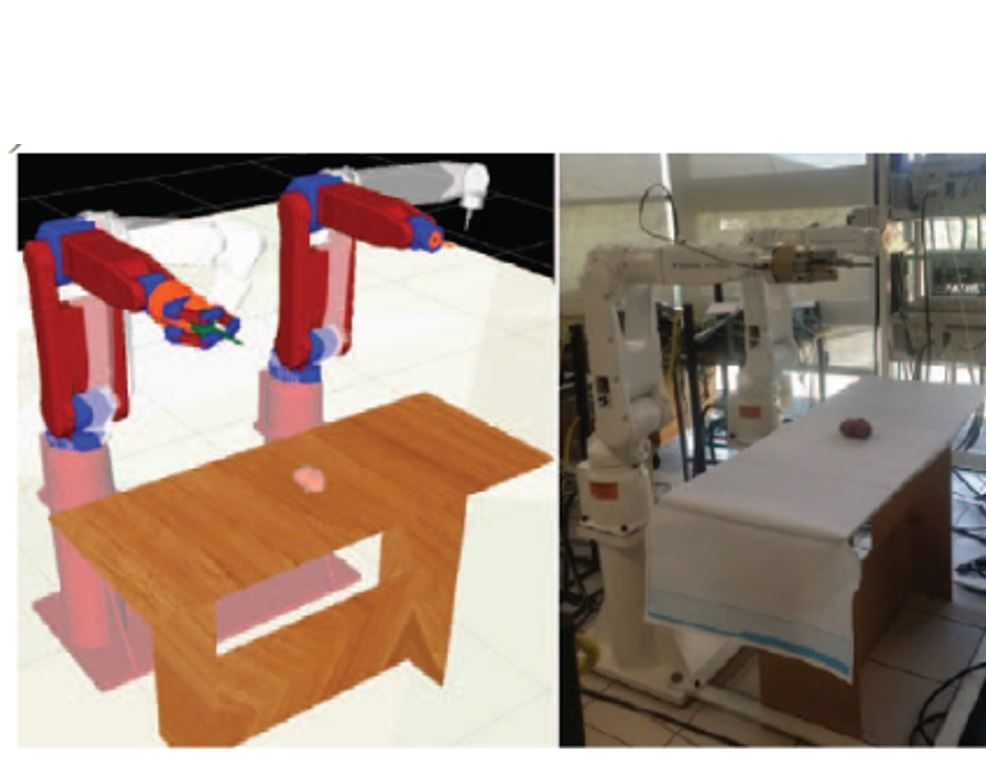
\includegraphics[width=0.45\textwidth]{01Introduccion/imagenes/04AntecedentesA.jpg}
        	}
        	\subfloat[
        	\label{fig:04AntecedentesB}]{%
        		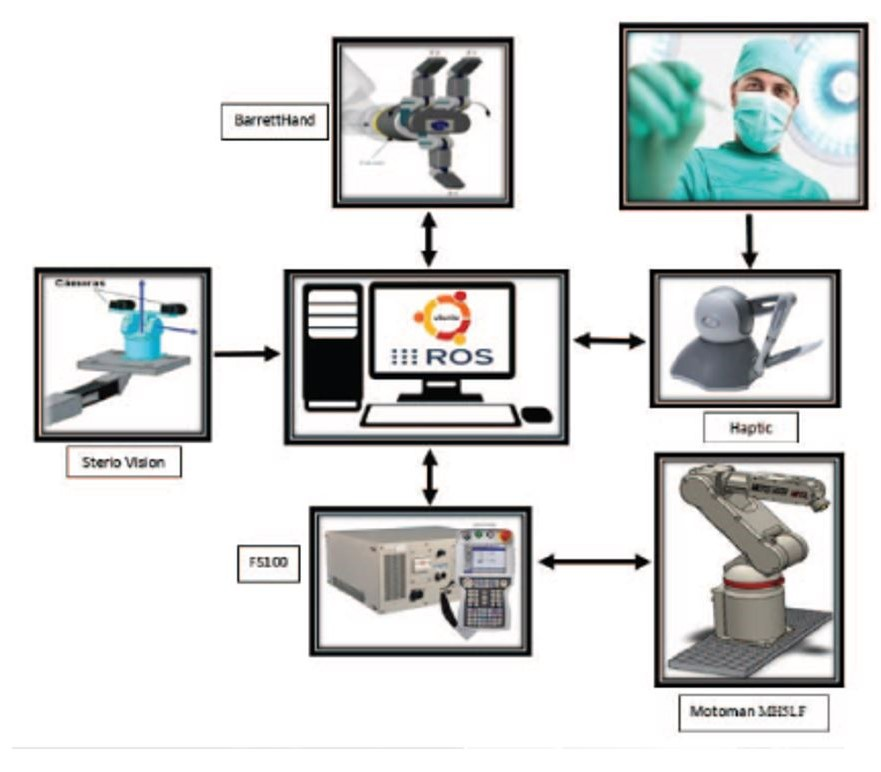
\includegraphics[width=0.45\textwidth]{01Introduccion/imagenes/04AntecedentesB.jpg}
        	}
        	\caption[Sistema de un robot medico.]{Sistema de un robot medico, (a)  Imágenes del sistema de brazos robot, (b) Diagrama del sistema médico robot. 
        	\label{fig:04Antecedentes}}
        \end{figure}
%        \begin{figure} [!htb]
%            \centering
%            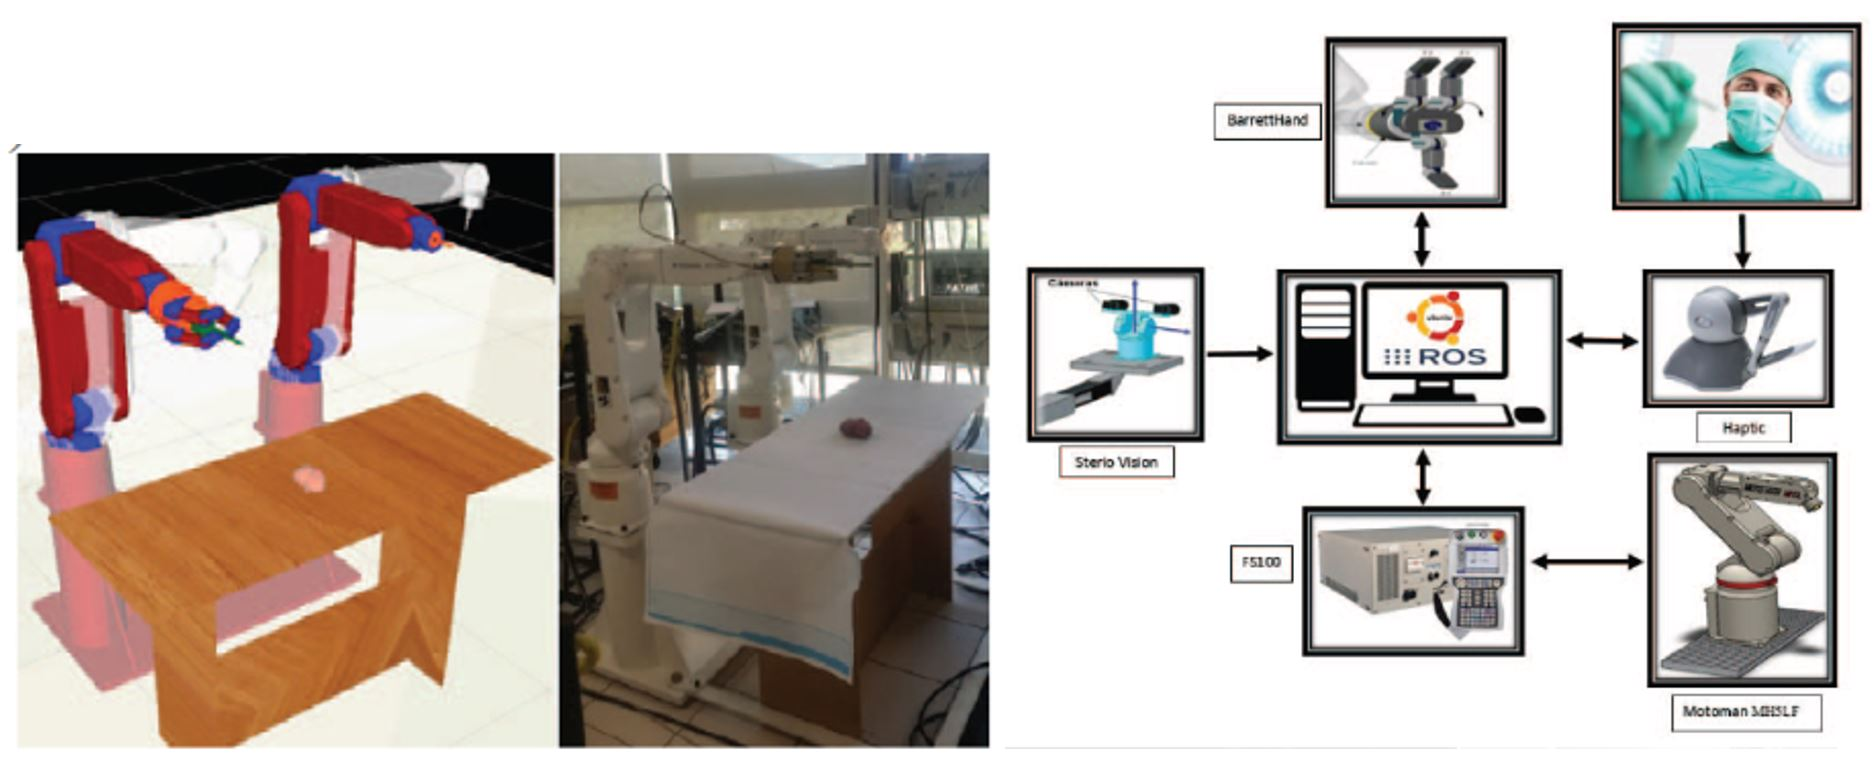
\includegraphics[width=1\textwidth]{01Introduccion/imagenes/04Antecedentes.jpg}
%            \caption{(izq.) Imágenes del sistema de brazos robot, (der.) Diagrama del sistema médico robot}% \cite{MedicalVisionAGC}} 
%            \label{fig:04Antecedentes}
%        \end{figure}
    
    
    \subsection{Visión por Computadora Mejorada con el Sensor Kinect de Microsoft }
    
        En el artículo con título “Enhanced Computer Vision with Microsoft Kinect Sensor: A Review” \cite{CompVisionKinect}, se describen algunas técnicas de Visión por Computadora con imágenes RGB que fueron modificadas o mejoradas usando el sensor Kinect como la que se muestra en la figura \ref{fig:02Antecedentes}, se describe una introducción al uso del Kinect en temas como el pre-procesamiento (usando la profundidad como filtro como se muestra en la figura \ref{fig:02AntecedentesC}), el seguimiento y reconocimiento de objetos (que permite dar su rotación y posición) y el reconocimiento de objetos en una escena (solo predice si existe un objeto).\\
        
        \begin{figure}[!htb]
        	\centering
        	\subfloat[
        	\label{fig:02AntecedentesA}]{%
        		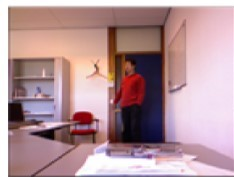
\includegraphics[width=0.33\textwidth]{01Introduccion/imagenes/02AntecedentesA.jpg}
        	}
        	\subfloat[
        	\label{fig:02AntecedentesB}]{%
        		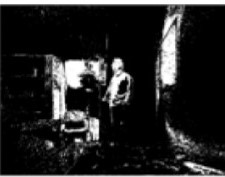
\includegraphics[width=0.33\textwidth]{01Introduccion/imagenes/02AntecedentesB.jpg}
        	}
        	\subfloat[
		    \label{fig:02AntecedentesC}]{%
		    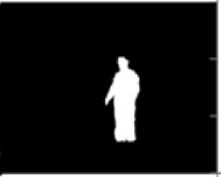
\includegraphics[width=0.33\textwidth]{01Introduccion/imagenes/02AntecedentesC.jpg}
			}
        	\caption[Segmentación de una imagen.]{Segmentación de una imagen, (a) Imagen RGB, (b) Máscara FG usando RGB, (c) Máscara FG usando profundidad.
        		\label{fig:02Antecedentes}}
        \end{figure}
    
%        \begin{figure}[!htb]
%            \centering
%            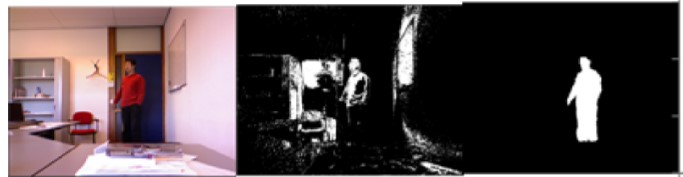
\includegraphics[width=1\textwidth]{01Introduccion/imagenes/02Antecedentes.jpg}
%            \caption{(izq.) imagen RGB, (cento) Mascara FG usando RGB, (der.) Mascara FG usando profundidad}%\cite{CompVisionKinect}} 
%            \label{fig:02Antecedentes}
%        \end{figure}
    
    \subsection{Mejorando la Clasificación y Detección de Objetos Basado en la Transformada de Hough y el Sensor Kinect}
    
        La transformada de Hough se usa en el procesamiento de imágenes ya que permite detectar formas simples como rectas, circunferencias o elipses. En el artículo titulado “Improving 3D Object Detection and Classification Based on Kinect Sensor and Hough Transform” \cite{CompVisionKinecthough}, se propone un algoritmo que usa puntos característicos y el espectro del color como dos procesos intercalados que cooperativamente reconocen objetos al estilo 2.5D, para automatizar el pre-procesamiento de una escena, en la figura \ref{fig:03Antecedentes} se observan las etapas del algoritmo.\\
    
        \begin{figure}[!htb]
            \centering
            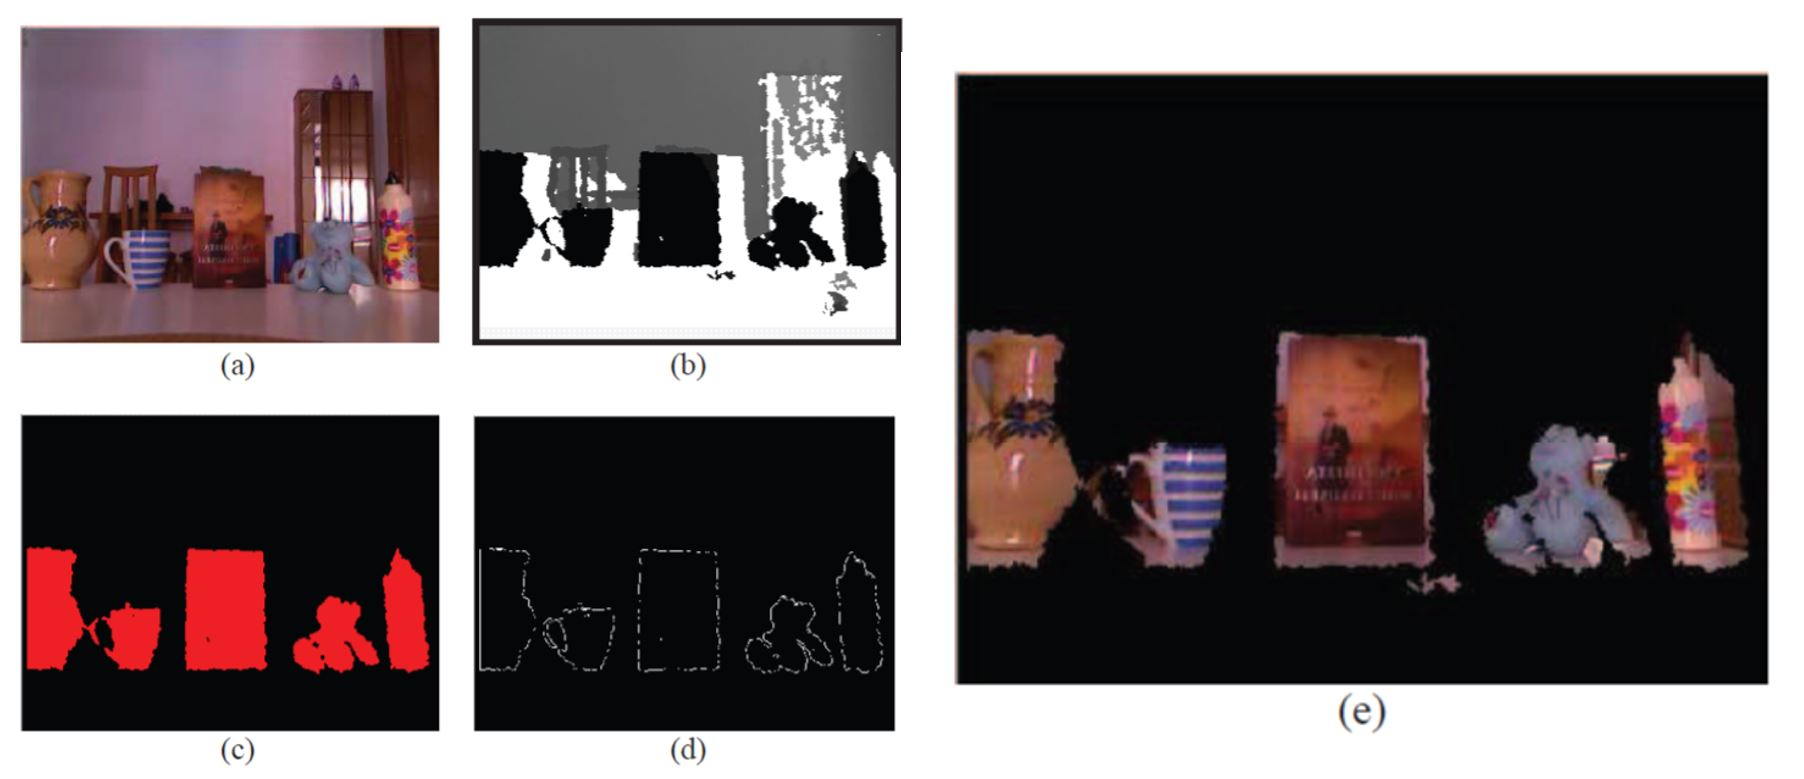
\includegraphics[width=1\textwidth]{01Introduccion/imagenes/03Antecedentes.jpg}
            \caption[Técnica de pre-procesamiento]{Técnica de pre-procesamiento, (a) Imagen RGB, (b) Imagen de profundidad, (c) Imagen binaria, (d) Filtro Canny, y (e) Segmentación}% \cite{CompVisionKinecthough}} 
            \label{fig:03Antecedentes}
        \end{figure}
    
    
    \subsection{Reconocimiento de Objetos Mediante Sensor 3D Kinect}
    
        En el proyecto titulado “Reconocimiento de Objetos Mediante Sensor 3D Kinect” \cite{RecoObj3d}, se utiliza un sensor Kinect 3D para obtener una malla de puntos y reconocer un grupo de objetos usando un clasificador basado en vectores. Obteniendo una nube de puntos del sensor 3D Kinect calculan los vectores normales al plano en cada punto del objeto, así como se muestra en la figura \ref{fig:01Antecedentes}, y se determina qué tipo de objeto es si cumple con las características dadas para cada figura. \\
        
        
        \begin{figure}[!htb] 
        	\centering
        	\subfloat[
        	\label{fig:01AntecedentesA}]{%
        		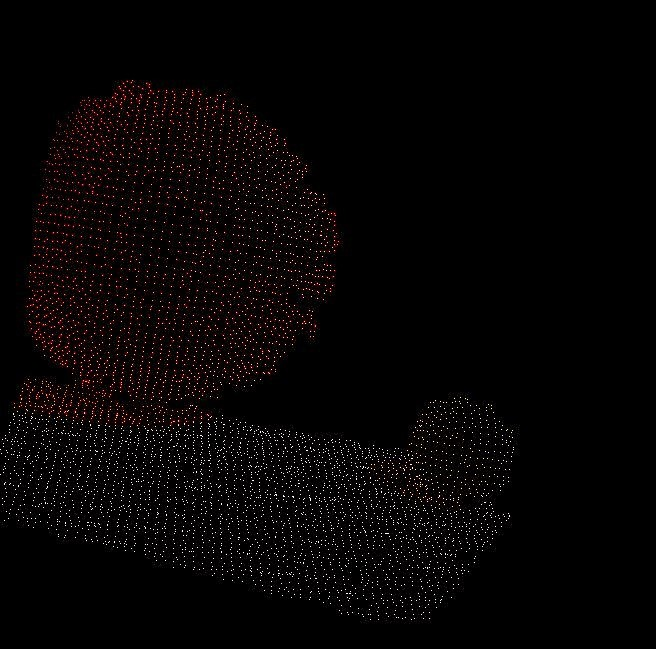
\includegraphics[width=0.45\textwidth]{01Introduccion/imagenes/01AntecedentesA.jpg}
        	}
        	\subfloat[
        	\label{fig:01AntecedentesB}]{%
        		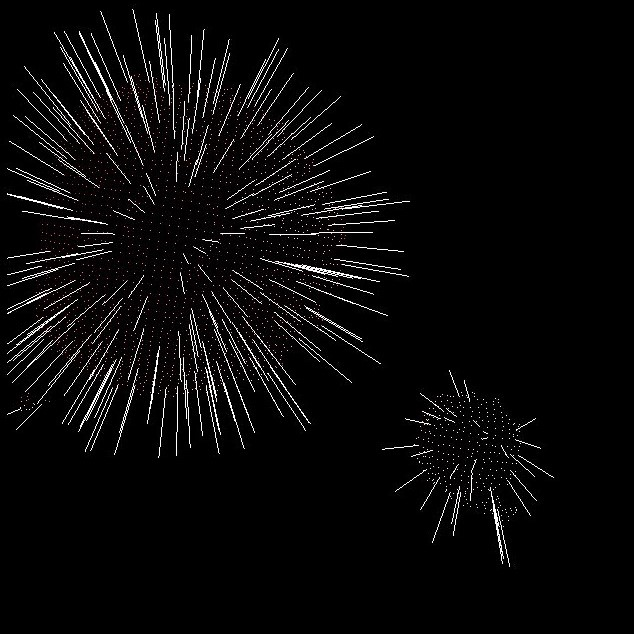
\includegraphics[width=0.45\textwidth]{01Introduccion/imagenes/01AntecedentesB.jpg}
        	}
        	\caption[Reconocimiento de objetos usando normales.]{Reconocimiento de objetos usando normales, (a)Nube de puntos obtenidos del sensor 3D Kinect, (b) Visualización de las normales calculadas. } 
        	\label{fig:01Antecedentes}
        \end{figure}
    
%        \begin{figure}[!htb] 
%            \centering
%            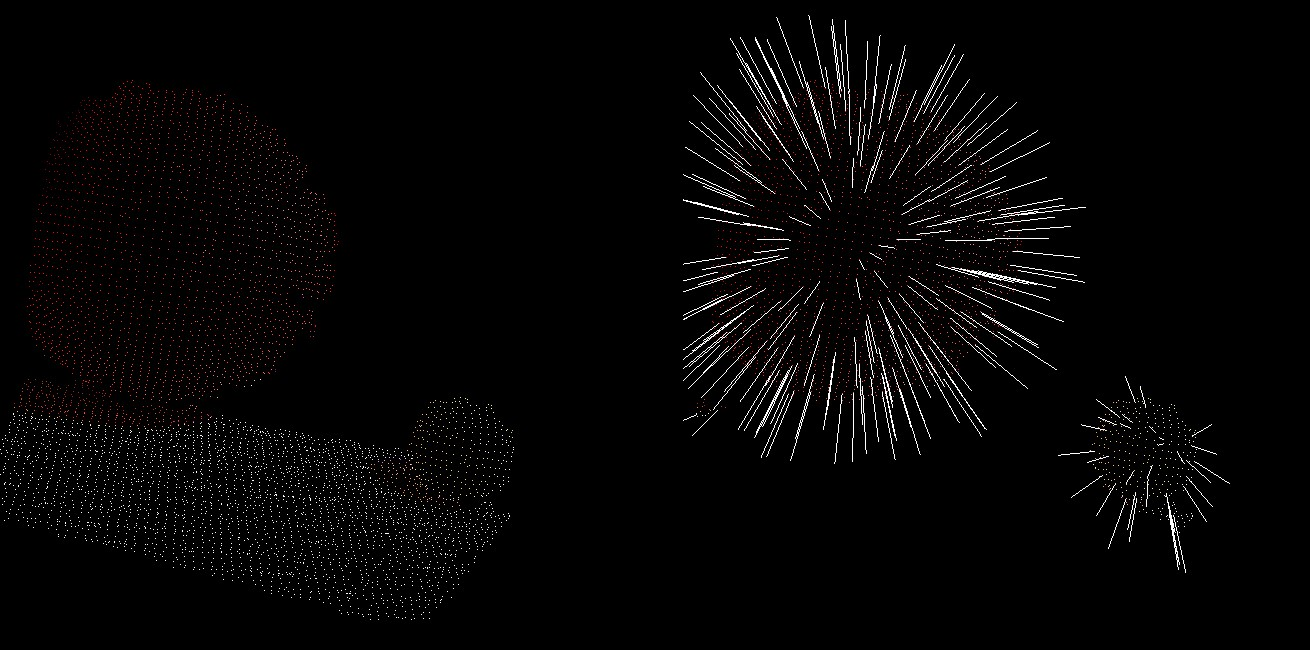
\includegraphics[width=.8\textwidth]{01Introduccion/imagenes/01Antecedentes.jpg}
%            \caption{(der.) Nube de puntos obtenidos del sensor 3D Kinect. (izq.) Visualización de las normales calculadas  }%\cite{RecoObj3d}}
%            \label{fig:01Antecedentes}
%        \end{figure}
    
    
    
    
    \subsection{Detección de Objetos en Nubes de Puntos Usando Álgebra Geométrica Conforme}
    
        En el trabajo “Object Detection in Point clouds Using Conformal Geometic Algebra” \cite{cilindrosAGC}, se usa el algoritmo RANSAC para detectar objetos con formas geométricas, así como también proponen varias formas de calcular cilindros usando AGC, primero usando una circunferencia extrudía sobre la normal del plano que pasa por el circulo y otra usando dos esferas como se muestra en la figura \ref{fig:05Antecedentes}.\\
        
        \begin{figure}[!htb] 
        	\centering
        	\subfloat[
        	\label{fig:05AntecedentesA}]{%
        		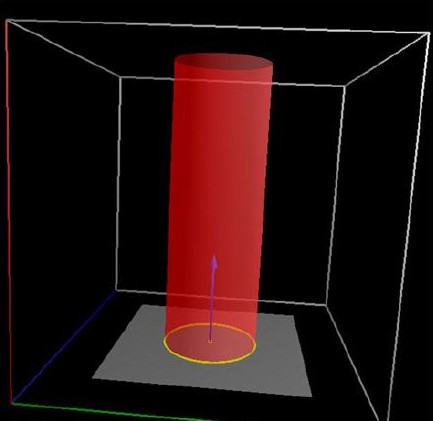
\includegraphics[width=0.45\textwidth]{01Introduccion/imagenes/05AntecedentesA.jpg}
        	}
        	\subfloat[
        	\label{fig:05AntecedentesB}]{%
        		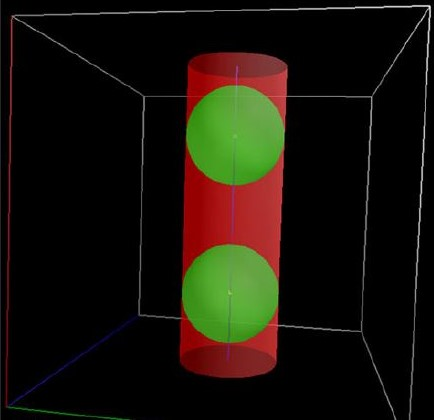
\includegraphics[width=0.45\textwidth]{01Introduccion/imagenes/05AntecedentesB.jpg}
        	}
        	\caption[Modelado de un cilindro usando AGC.]{Modelado de un cilindro usando AGC, (a) Cilindro construido usando circulo y su normal, (b) Cilindro construido con dos esferas y la linea que une sus centros.} 
        	\label{fig:05Antecedentes}
        \end{figure}
        
%        \begin{figure}[!htb] 
%            \centering
%            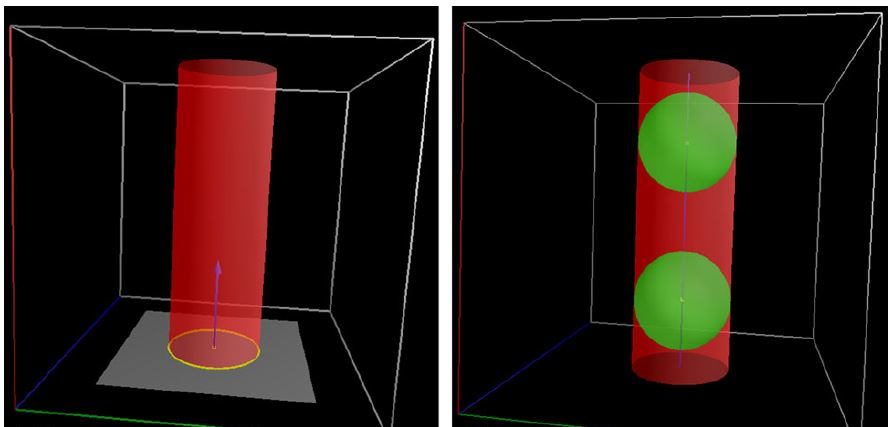
\includegraphics[width=.8\textwidth]{01Introduccion/imagenes/05Antecedentes.jpg}
%            \caption{(izq.) Cilindro construido usando circulo y su normal, (der.) Cilindro construido con dos esferas y la linea que une sus centros.} 
%            \label{fig:05Antecedentes}
%        \end{figure}
        
    
